\documentclass[Orbiter Developer Manual.tex]{subfiles}
\begin{document}

\section{Planets and moons}
Orbiter allows to create new planets or planetary systems in a few simple steps. To create a new planet, you need to do the following:

\begin{itemize}
\item find or create a surface texture map
\item optionally, find or create texture maps for a cloud layer, for a land/sea mask, and for night lights
\item convert the texture map(s) into Orbiter's .tex format by invoking pltex
\item create a configuration file (.cfg) in the Config subfolder, containing physical and orbital planet parameters.
\item Add an entry for the planet in the configuration file of the planetary system (e.g. Sol.cfg).
\item Optionally, create a DLL plugin module to allow detailed control of planet movement and atmosphere definition.
\end{itemize}


\subsection{Planetary textures}
\label{ssec:planetery_tex}
This section describes the format introduced in Orbiter 2016 to define the surface textures, surface elevations and cloud layers for planetary bodies (planets, moons, asteroids, etc.)\\
This is a more powerful planetary texturing mechanism than previous releases that provides

\begin{itemize}
\item higher resolution levels
\item support for surface elevation modelling
\item a consistent hierarchical quad-tree implementation for level-of-detail (LOD) mapping over a large resolution range
\end{itemize}

\noindent
The legacy texture mapping used in pre-Orbiter 2016 releases is still supported by Orbiter for backward compatibility, but its use in new planet texture projects is discouraged.
\\
To configure a planet for use of the new surface texture format, its configuration file\\
\indent Config\textbackslash <\textit{planet name}>.cfg\\
must contain the following line:

\begin{lstlisting}[language=OSFS]
TileFormat = 2
\end{lstlisting}

\noindent
If missing, the legacy format is assumed. Likewise, if a cloud layer is present and is defined in the new format, the configuration file must contain

\begin{lstlisting}[language=OSFS]
CloudFormat = 2
\end{lstlisting}

\noindent
otherwise a cloud layer defined in the legacy format is assumed.\\
The MaxPatchResolution tag can be used to specify the maximum resolution level Orbiter will use for rendering the planet surface. This can be higher than than the maximum resolution defined in the texture quadtree, in which case Orbiter interpolates the missing high-resolution tile from the highest available resolution ancestor tile. This can be useful for providing a smoother surface representation (in particular for elevation data). The maximum supported value is 19. If the MaxPatchResolution value is set to less than the highest resolution level supported by quadtree nodes, then the higher resolution tiles are not used for rendering.\\
Likewise, the MaxCloudResolution tag can be used to specify the maximum resolution level for cloud tiles (the MinCloudResolution tag should always be set to 1).


\subsubsection{The file layout}
\label{sssec:tile_file_layout}
The files which describe the surface and cloud layer of a planetary body are located in a subdirectory\\
\indent Textures\textbackslash <\textit{planet name}>\\
relative to the Orbiter root directory, where <\textit{planet name}> is a place holder for the name of the celestial body, e.g. Textures\textbackslash Earth.\\
The folder for each celestial body contains one or several sub-folders for various layers. Currently Orbiter supports the following layers:

\begin{itemize}
\item Surf $\Rightarrow$ Surface textures
\item Mask $\Rightarrow$ Water masks and night light textures
\item Elev $\Rightarrow$ Surface elevation maps
\item Elev\_mod $\Rightarrow$ Surface elevation modifiers
\item Label $\Rightarrow$ Labels for surface features
\item Cloud $\Rightarrow$ Cloud textures
\end{itemize}

\noindent
Only the Surf layer is required. All other layers are optional.\\
The files for each layer are arranged in a hierarchical quad-tree that is reflected by the folder structure within each layer.\\
Each layer can be represented by multiple resolution levels ($\geq$ 1) up to a maximum level of currently 19. The different resolution levels are split into subdirectories represented by 2-digit folder names. For example,\\
\indent Textures\textbackslash Earth\textbackslash Surf\textbackslash 08\\
contains the level-8 surface textures for Earth.\\
Each resolution level is further subdivided into latitude bands ($\geq$ 0), represented by 6-digit subdirectories, e.g.\\
\indent Textures\textbackslash Earth\textbackslash Surf\textbackslash 08\textbackslash 000005\\
contains the surface textures for latitude band 5 at resolution 8. The range of latitude bands \textit{ilat} depends on the resolution level \textit{n}:\\
\indent 0 $\leq$ \textit{ilat} $\leq$ \textit{nlat} - 1  with  \textit{nlat} = 2$^{n-4}$  (n $\geq$ 4)\\
where \textit{ilat} = 0 contains the northernmost latitude band, and \textit{ilat} = \textit{nlat} - 1 contains the southernmost latitude band.\\
Each latitude band subfolder contains the files for the tiles of that latitude band. Each file has a 6-digit file name representing the longitude index of the file, and an extension depending on the layer type. The range of longitude indices (\textit{ilng}) also depends on the resolution level:\\
\indent 0 $\leq$ \textit{ilng} $\leq$ \textit{nlng} - 1  with  \textit{nlng} = 2$^{n-3}$  (n $\geq$ 4)\\
where \textit{ilng} = 0 contains the westernmost longitude tile (left edge at longitude 180° W), and \textit{ilng} = \textit{nlng} - 1 contains the easternmost longitude tile (right edge at longitude 180° E).\\
For example the Earth surface texture tile for resolution level 8, latitude index 5 and longitude index 7 is located in\\
\indent Textures\textbackslash Earth\textbackslash Surf\textbackslash 08\textbackslash 000005\textbackslash 000007.dds


\subsubsection{The quadtree structure}
\label{sssec:quadtree_struct}
The planet surface is divided into tiles along latitude and longitude boundaries. Each tile at resolution level n can be divided into 2x2 sub-tiles at resolution level \textit{n} + 1. Each tile can therefore be represented as a \textit{node} in a quadtree structure with one parent (except for the root tiles) and up to four children.\\
The root of the tile quadtree consists of two tiles at resolution level 4:\\
\indent Textures\textbackslash <\textit{planet name}>\textbackslash <\textit{layer}>\textbackslash 04\textbackslash 000000\textbackslash 000000.<\textit{ext}>\\
\indent Textures\textbackslash <\textit{planet name}>\textbackslash <\textit{layer}>\textbackslash 04\textbackslash 000000\textbackslash 000001.<\textit{ext}>\\
where file 04\textbackslash 000000\textbackslash 000000.<\textit{ext}> contains the western hemisphere (-180° $\leq$ \textit{lng} $\leq$ 0° and -90° $\leq$ \textit{lat} $\leq$ +90°), and file 04\textbackslash 000000\textbackslash 000001.<ext> contains the eastern hemisphere (0° $\leq$ \textit{lng} $\leq$ +180° and -90° $\leq$ \textit{lat} $\leq$ +90°).\\
The area covered by tile 04\textbackslash 000000\textbackslash 000000.<\textit{ext}> can be split into four subtiles at level 5:\\
\indent Textures\textbackslash <\textit{planet name}>\textbackslash <\textit{layer}>\textbackslash 05\textbackslash 000000\textbackslash 000000.<\textit{ext}>\\
\indent Textures\textbackslash <\textit{planet name}>\textbackslash <\textit{layer}>\textbackslash 05\textbackslash 000000\textbackslash 000001.<\textit{ext}>\\
\indent Textures\textbackslash <\textit{planet name}>\textbackslash <\textit{layer}>\textbackslash 05\textbackslash 000001\textbackslash 000000.<\textit{ext}>\\
\indent Textures\textbackslash <\textit{planet name}>\textbackslash <\textit{layer}>\textbackslash 05\textbackslash 000001\textbackslash 000001.<\textit{ext}>\\
In general, a tile at resolution level n with latitude and longitude indices [\textit{n}, \textit{ilat}, \textit{ilng}] has subtiles\\
\indent [\textit{n} + 1, 2 \textit{ilat}, 2 \textit{ilng}] $\rightarrow$ [\textit{n} + 1, 2 \textit{ilat}, 2 \textit{ilng} + 1]\\
\indent [\textit{n} + 1, 2 \textit{ilat} + 1, 2 \textit{ilng}] $\rightarrow$ [\textit{n} + 1, 2 \textit{ilat} + 1, 2 \textit{ilng} + 1]\\
at resolution level \textit{n} + 1.\\
The latitude and longitude range covered by tile [\textit{n}, \textit{ilat}, \textit{ilng}] is given by

\[ -180^{\circ} + \frac{360^{\circ}}{nlng}ilng \leq lng \leq -180^{\circ} + \frac{360^{\circ}}{nlng}(ilng + 1), \quad nlng = 2^{n - 3} \]
\[ 90^{\circ} - \frac{180^{\circ}}{nlat}(ilat + 1) \leq lat \leq 90^{\circ} - \frac{180^{\circ}}{nlat}ilat, \quad nlat = 2^{n - 4} \]

\noindent
For example, tile [n = 8, ilat = 5, ilng = 7] spans the area

\[ 22.5^{\circ} \leq lat \leq 33.75^{\circ}, \quad -101.25^{\circ} \leq lng \leq -90^{\circ} \]

\noindent
Resolution levels 1, 2 and 3 are not part of the quadtree. They cover the entire planet surface at different resolution levels. For example, for the Surf layer, tile 01\textbackslash 000000\textbackslash 000000.dds contains the planet surface as a 128x128 pixel texture, 02\textbackslash 000000\textbackslash 000000.dds contains the planet surface as a 256x256 pixel texture, and  03\textbackslash 000000\textbackslash 000000.dds contains the planet surface as a 512x512 pixel texture.

\begin{figure}[H]
	\centering
	\subfigure{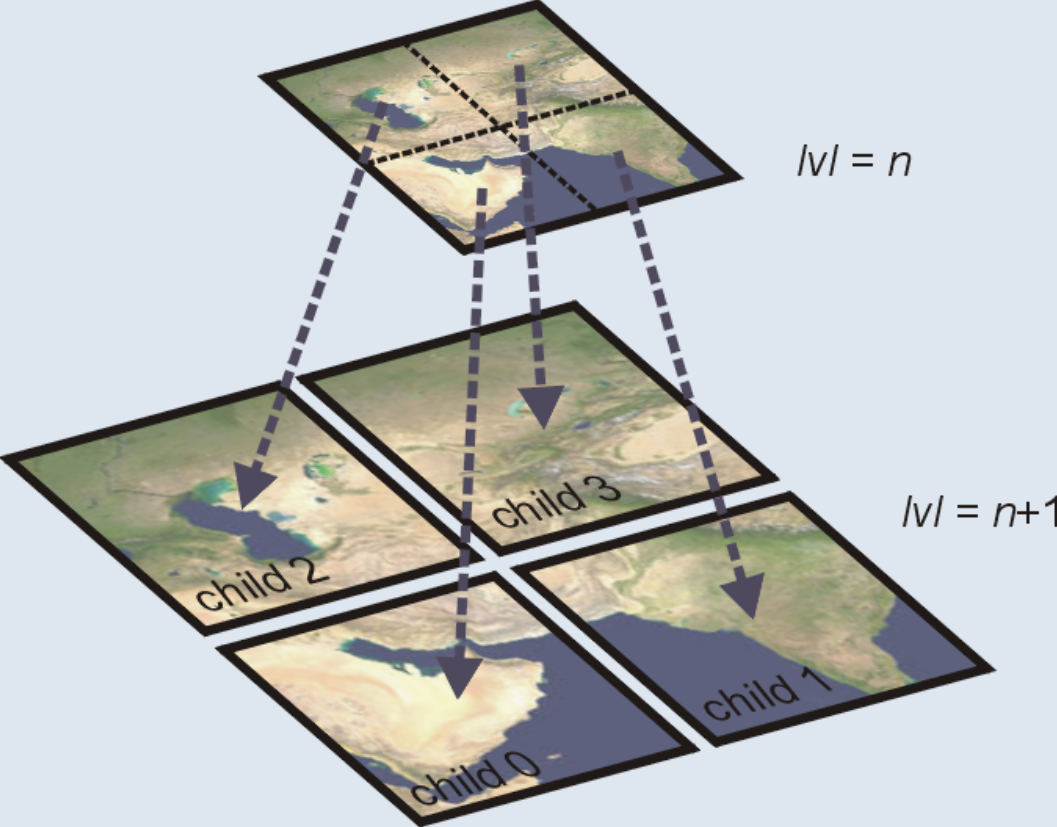
\includegraphics[width=0.5\textwidth]{quad_tree_tile.png}}
	\caption{Quadtree tile subdivision and child tiles at the next resolution level.}
\end{figure}

\noindent
The quadtree doesn't need to be populated completely. Missing tiles are interpolated by Orbiter from a sub-area of an ancestor tile. The quadtree is also allowed to contain gaps, that is, it can contain high-resolution tiles of an area (e.g. a surface base) even if some of the ancestor tiles are missing from the tree, so that there is no unbroken chain to the quadtree root.\\
The minimum requirement is the presence of all tiles for resolution levels 1 to 4 for a given layer, i.e. the global tiles (level 1-3) and the quadtree root (level 4) must be present. All higher resolution quadtree tiles are optional. The maximum currently supported resolution level is 17 for elevation layers (Elev and Elev\_mod), and level 19 for all other layers.



\subsubsection{Layer types}
The following layer types are currently supported by Orbiter:\\

\noindent
\textbf{Surf layer}\\
The Surf layer contains the surface texture of a planet, where the file for each tile is a 512x512 pixel bitmap in DXT1 format (no transparency). You can for example use the Utils\textbackslash DxTex.exe (DirectX Texture Tool) utility to convert a bitmap to DXT1 format. You can also use the Utils\textbackslash plsplit64.exe utility to convert a planetary map in cylindrical projection to a set of files at a given resolution level.\\

\noindent
\textbf{Mask layer}\\
The Mask layer contains the planet water mask (for rendering specular reflection of water surfaces) and night light texture, if applicable, in a combined  512x512 pixel DXT1 texture file (1-bit transparency). The RGB channels of the texture provide the night light information, while the 1-bit alpha channel provides the water mask (alpha = 0: water, alpha = 1: land). Due to a limitation of the DXT1 format, pixels with alpha = 0 do not contain RGB information. Therefore, night lights cannot be defined on water surfaces.\\
A planet with neither night lights nor specular reflection surfaces does not need to provide a Mask layer.\\

\noindent
\textbf{Elev layer}\\
The Elev layer contains files defining the surface elevation of a tile in a custom format (*.elv, see section \ref{sssec:elev_tile_format}). Planets which do not define an Elev layer are represented as spheres.\\

\noindent
\textbf{Elev\_mod layer}\\
The Elev\_mod layer allows to modify tile elevations without the need to modify the original Elev files. The Elev\_mod layer can be used e.g. for editing the elevations at surface bases (flattening runways, etc.). The files are in a custom format (*.elv, see section \ref{sssec:elev_tile_format}). A tile in the Elev\_mod layer can only modify an existing tile in the Elev layer, not create a new tile. Therefore, for each tile in the Elev\_mod layer, the corresponding tile in the Elev layer must exist.\\

\noindent
\textbf{Cloud layer}\\
The Cloud layer contains the tiles for a global cloud layer in 512x512 pixel DXT5 format, containing colour and transparency information. Planets without clouds don't define this layer.\\

\noindent
\textbf{Label layer}\\
The Label layer contains positions and labels for surface features such as cities, mountains, craters, landing sites, etc. See section \ref{sssec:label_tile_format} for details.


\subsubsection{Compressed archive layer format}
\label{sssec:compress_archive_layer}
The quadtree tile format described in sections \ref{sssec:tile_file_layout} and \ref{sssec:quadtree_struct} consists of individual files for each tile. This can lead to a very large number of files and a complex directory structure, which is often not desirable. Therefore, Orbiter alternatively supports a compressed archive layer format, where all files for a given planet and layer are merged into a single file.\\
The archive files can exist alongside the directory tree containing the individual tile files (the "cache"). Orbiter can be configured to read only from the cache, only from the archive, or from both (first trying the cache, then the archive). To set these preferences, use the\\
\indent Extra | Visualisation parameters | Planet rendering options | Tile sources\\
controls in the Orbiter Launchpad dialog (for the inline graphics version), or the corresponding client-specific controls for external graphics clients.\\
Compressed archive files have a custom format. They consist of a header, a table of contents (TOC) representing the tree structure, and the compressed and concatenated tile files. Archive files have the extension .tree (to signify that they contain quadtree data). They are located in\\
\indent Textures\textbackslash <\textit{planet name}>\textbackslash Archive\\
with

\begin{itemize}
\item Surf.tree $\Rightarrow$ Surf layer
\item Mask.tree $\Rightarrow$ Water mask and night light layer
\item Elev.tree $\Rightarrow$ Elevation layer
\item Elev\_mod.tree $\Rightarrow$ Elevation modification layer
\item Cloud.tree $\Rightarrow$ Cloud layer
\end{itemize}

\noindent
A layer archive (.tree) file consists of a header, TOC and compressed node data. The file header has the following format:

\begin{lstlisting}
struct ZtreeHeader
{
	BYTE magic[4];// file ID and version ('T', 'X', 1, 0)
	DWORD size;// header size [bytes] (48)
	DWORD flags;// bit flags (currently ignored)
	DWORD dataOfs;// data block offset (header + TOC)
	__int64 dataLength;// total length of compressed data block
	DWORD nodeCount;// total number of tree nodes
	DWORD rootPos1;// index of level-1 tile
	DWORD rootPos2;// index of level-2 tile
	DWORD rootPos3;// index of level-3 tile
	DWORD rootPos4[2];// index of level-4 tiles (quadtree roots)
};
\end{lstlisting}

\noindent
where dataOfs specifies the offset of the data block from the file start (= size of header + table of contents), dataLength is the size of the data block (= file size - dataOfs) and nodeCount is the number of entries in the TOC.\\
rootPos1, rootPos2, rootPos3 are the indices of the level 1, 2 and 3 tiles in the TOC, respectively, and rootPos4 are the indices of the two level 4 quadtree roots in the TOC. If any of these is not present in the TOC, the value is set to (DWORD)-1.\\
The header is followed by the TOC, consisting of a list of nodeCount quadtree node descriptors. A descriptor is given by

\begin{lstlisting}
struct TreeNode
{
	__int64 pos;// file position of node data
	DWORD size;// data block size [bytes]
	DWORD child[4];// array index positions of the children
};
\end{lstlisting}

\noindent
where pos is the node's data position in the file relative to the beginning of the data block, size is the node's decompressed data size, and child contains the indices of the four descendants, where (DWORD)-1 terminates the branch.\\
The compressed data size of node i can be inferred from node[i + 1].pos - node[i].pos, where node[i + 1].pos must be replaced with dataLength for the last node.\\
Note that the TOC may contain nodes without data block, if they are required to provide connectivity across gaps to higher-resolution descendants. The uncompressed size of such dummy nodes is set to 0.\\
The TOC is followed by the compressed node data, following the same order as the TOC. The data for each node are compressed individually, using the zlib "deflate" method with Z\_DEFAULT\_COMPRESSION setting, essentially providing a gz compression format for each individual data block.


\subsubsection{Utilities}
The Utils folder contains some tools to assist with planetary texture management and editing.\\
\\
\textbf{tileedit}\\
Utils\textbackslash tileedit.exe is a tile viewer that is useful for navigating the tile quadtree. It can display multiple layers side by side, and has some basic editing capabilities for elevation tiles.

\begin{figure}[H]
	\centering
	\subfigure{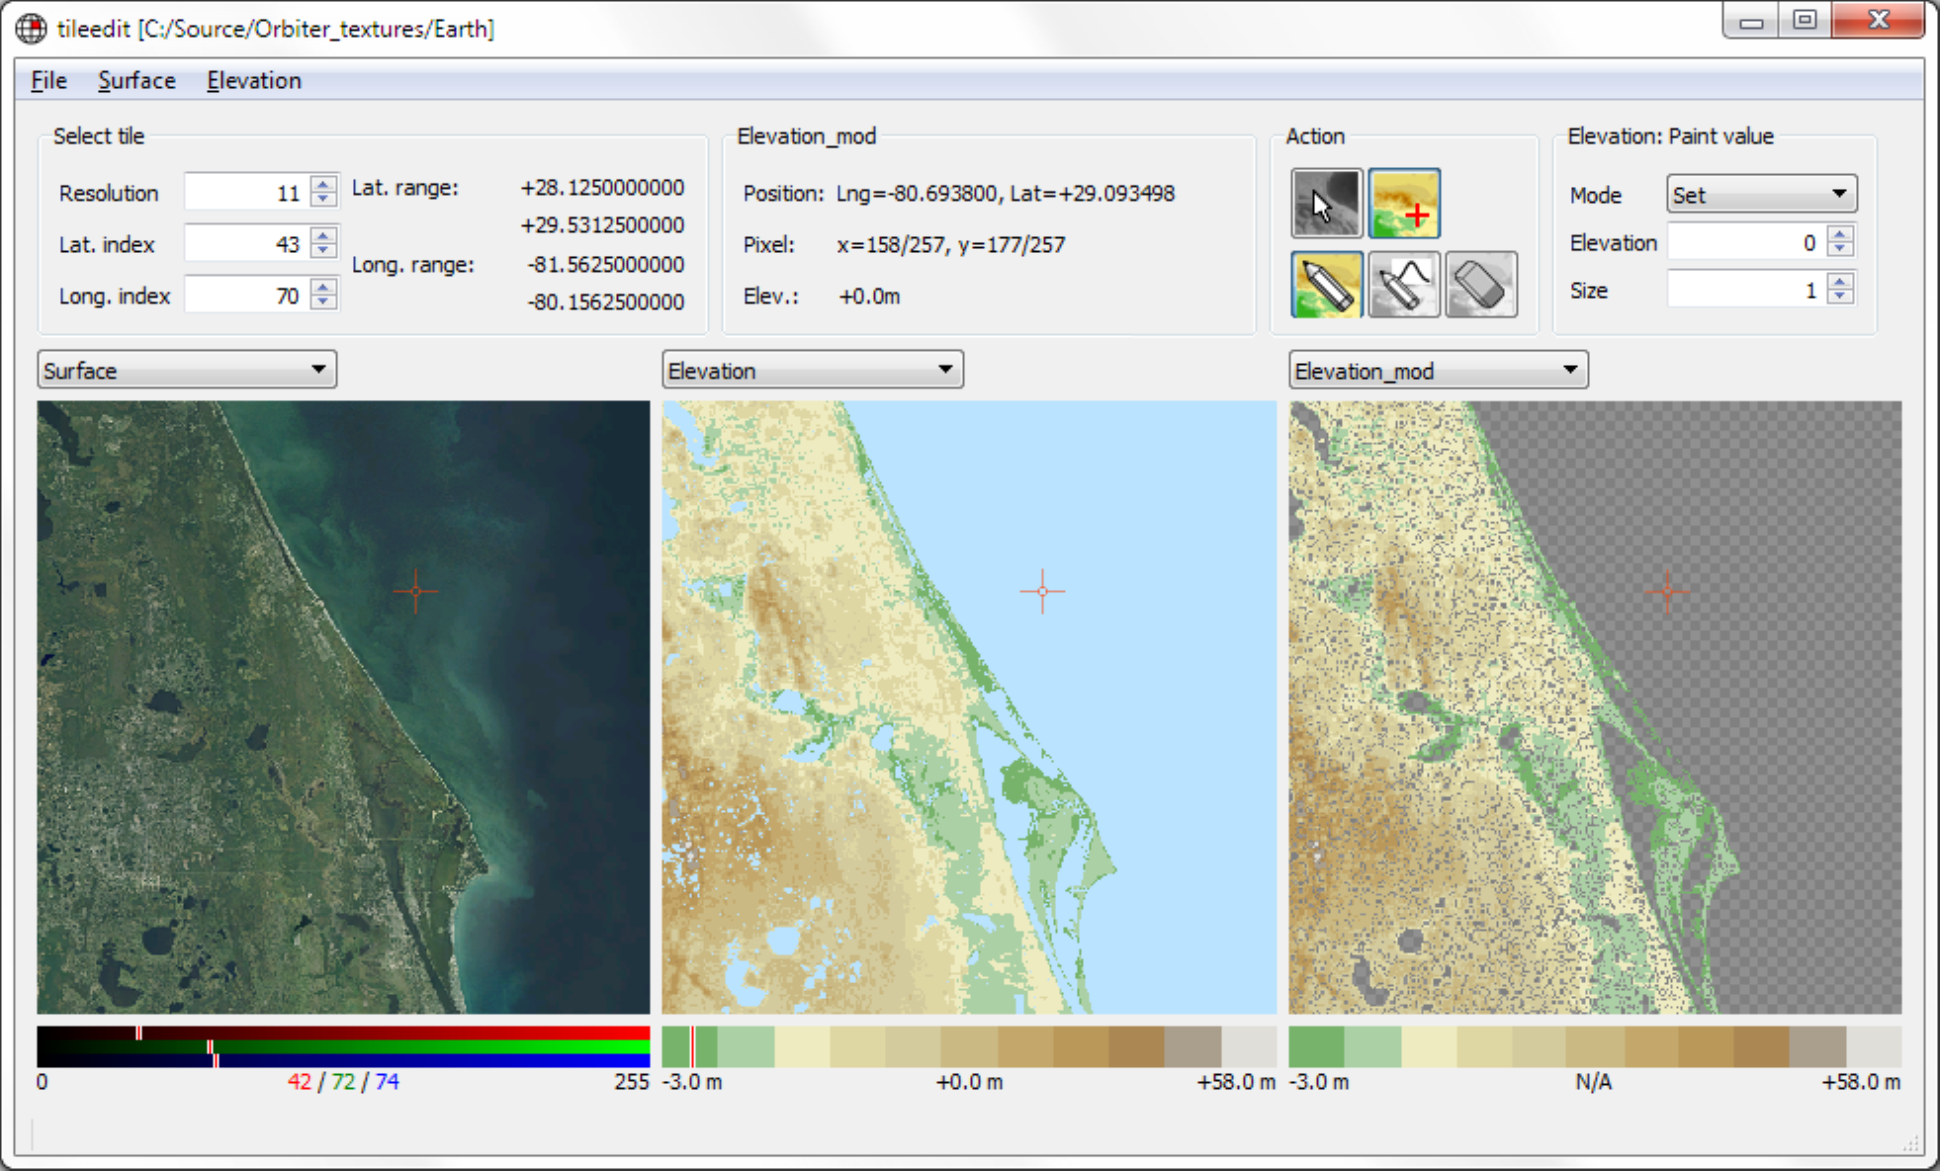
\includegraphics[width=0.99\textwidth]{tileedit.png}}
\end{figure}

\noindent
Tileedit can be configured to read from the quadtree cache or from a compressed archive (under File | Configure). Any modifications are always written as individual tiles into the cache directory structure. Therefore, changes will only be visible in Orbiter if it uses the cache (see section \ref{sssec:compress_archive_layer}), unless the changes are merged into the archive afterwards (see "texpack" below).\\
After launching tileedit, select a planet with File | Open and navigate to the root folder of a planet texture directory, for example\\
\indent Textures\textbackslash Earth\\
Then click Select Folder. This will open the Earth textures at the lowest resolution (level 1). The three map panels will show three surface layers, e.g. Surface, Elevation and water mask. Note that some layers may not be defined at level 1, and show a black square.\\
\\
Move the mouse over one of the map panels until it is surrounded by a red square. Click on it to proceed to the next higher level. At level 3 you can click on the western or eastern hemisphere to progress to one of the level 4 tiles. At higher levels you can click on one of the four quadrants to proceed to a child tile.\\
Moving the mouse to the centre of the image until an "X" appears and clicking will return to the parent tile.\\
Moving the mouse towards one of the edges until an arrow appears and clicking will move the view to the corresponding neighbour tile.\\
You can also select a tile directly by entering the resolution level, latitude and longitude index in the index fields at the top left.\\
Note that tileedit will display a representation of the selected tile even if there is no file for that tile. Tileedit then interpolates a sub-region of an ancestor tile. You can see the tile designation in the top left corner of the map panel when the mouse is hovering over it, e.g 16\textbackslash 000887\textbackslash 004095 . If the map was synthesized from an ancestor tile, the source tile is displayed below it in brackets, e.g. [13\textbackslash 000110\textbackslash 000511].\\
\\
You can select different layers from the drop-down box above each of the map panels.\\
\\
Tileedit allows to modify elevation data.

\begin{itemize}
\item Navigate to the tile you want to modify
\item Make sure that one of the map panels shows the elevation layer
\item Under the Action tab in the user interface area, click the Edit elevation icon.
\item Pick one of the paint modes, and adjust any option-specific parameters
\item Move the mouse over the elevation image and click to start drawing
\end{itemize}

\noindent
Changes will be written to the Elev\_mod layer rather than the original Elev layer. Having the Elevation\_mod layer open next to the Elevation layer can give a better of what parts of the map have been modified. Note that the Elevation map shows the modifications merged with any unmodified parts of the original map.\\
You can edit the elevation layer even by clicking in a different map panel (e.g. the Surface map). This gives better control for synchronising elevation modifications with surface features, e.g. for flattening a runway or similar. Cross hairs appear on all three map panels when in editing mode to provide an additional visual cue.\\
You can undo all modifications to an elevation tile by deleting the corresponding file in the Elev\_mod layer cache directory.\\
\\
\textbf{plsplit}\\
Utils\textbackslash plsplit.exe is an interactive command line utility that allows a planetary surface bitmap to be split into individual tile files at a specific resolution level.\\
The user must provide the surface bitmap in BMP (24-bit) format at the correct resolution. To generate multiple resolution levels, plsplit must be run multiple times with surface bitmaps at the corresponding resolutions.\\
The source bitmap must represent the global planet surface or a rectangular sub-area in cylindrical projection (longitude along horizontal axis, latitude along vertical axis). If the entire planet surface is to be processed from a single bitmap, the bitmap must cover longitude from -180° (left edge) to +180° (right edge) and latitude from -90° (bottom edge) to +90° (top edge).\\
To create a level-4 tile set, the source bitmap for global coverage must be 1024x512 pixels in size. For each subsequent resolution level, the bitmap must double in size both horizontally and vertically.\\
In practice, start with the highest resolution supported by your source map. If the size of the map is not a power of 2, use an image editing tool to interpolate to the closest power of 2. Then repeat reducing the size of the bitmap by a factor of 2 using an image editing tool to create the next lower level all the way to level 4 (1024x512). Levels 3, 2 and 1 must be created from source maps 512x512, 256x256 and 128x128, respectively.\\
If the planet surface contains water areas with specular reflections or night lights, the corresponding source bitmaps for these must also be provided to plsplit in the same sizes as the surface map.\\
\\
\textbf{texpack}\\
Utils\textbackslash texpack.exe is a command line utility which packs individual tile files from the cache directory tree into a compressed archive and stores it in the Archive subfolder of the planet texture directory. Please be aware that for very large tile trees the packing operation can take a long time (several hours).


\subsubsection{Elevation tile file format}
\label{sssec:elev_tile_format}
Orbiter uses a custom file format (*.elv) for encoding tile elevation data. The data file uses a binary format consisting of a header and the raw elevation data.

\begin{figure}[H]
	\centering
	\subfigure{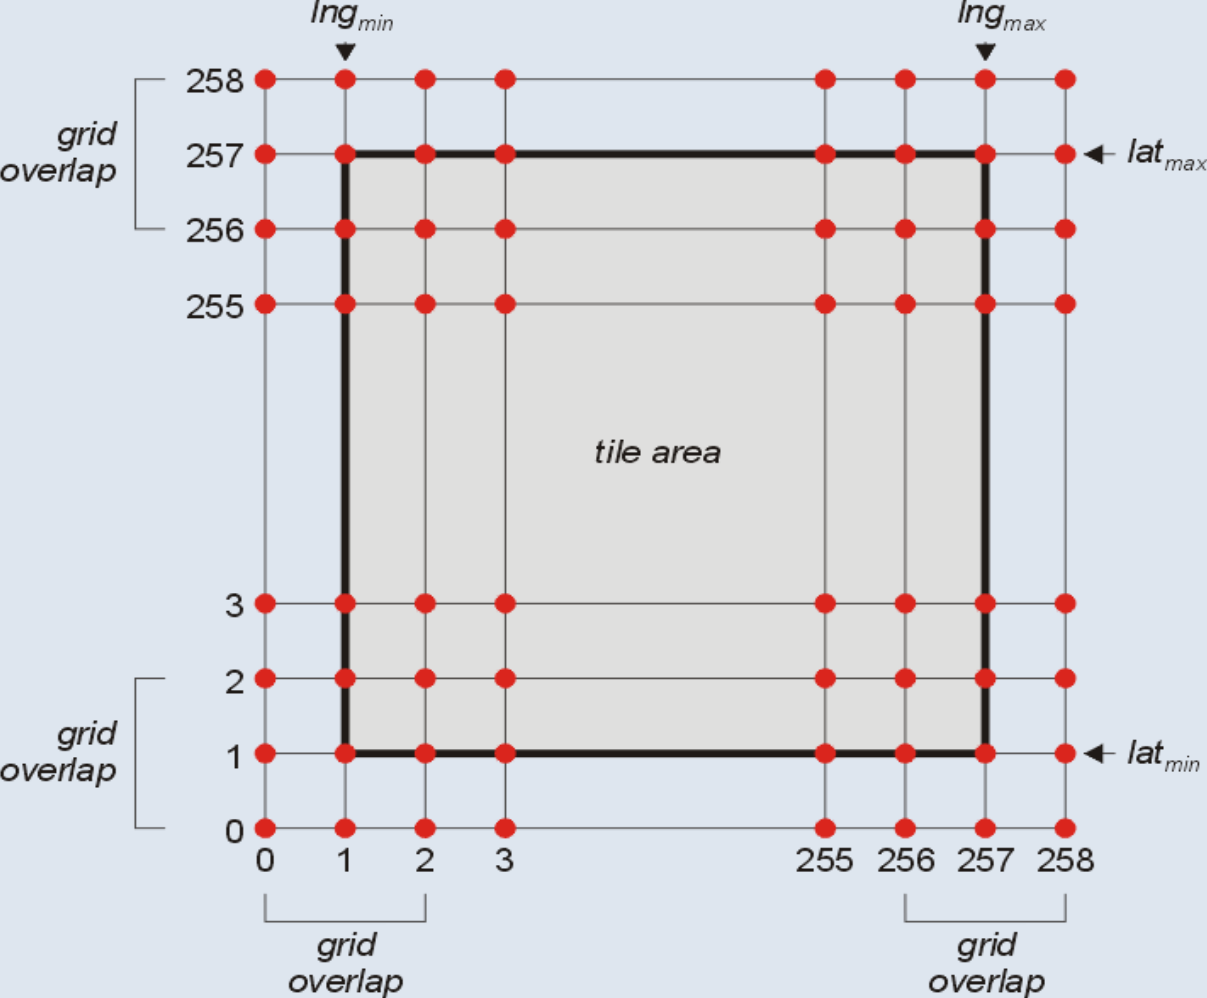
\includegraphics[width=0.5\textwidth]{tile_elev_grid.png}}
	\caption{Tile elevation grid and surface cover}
\end{figure}

\noindent
Each tile file represents a 259x259 grid of elevation points (with row and column indices 0-258). Column 1 represents the left edge of the tile, column 257 represents the right edge of the tile. Columns 0 and 258 are padding and are used for computing surface normals at the edges. This means that columns 0, 1 and 2 are shared with the left neighbour, and columns 256, 257 and 258 are shared with the right neighbour. The same is true for the top and bottom neighbours. The values stored for the shared nodes must be consistent between neighbouring tiles, otherwise edge artefacts can occur.\\
The file header has the following structure:

\begin{lstlisting}
struct ELEVFILEHEADER// file header for patch elevation file
{
	char id[4];// ID string + version ('E','L','E',1)
	int hdrsize;// header size (100 expected)
	int dtype;// data format (0=flat, no data block; 8=uint8, -8=int8,
				//16 =uint16, -16=int16)
	int xgrd,ygrd;// data grid size (259 x 259 expected)
	int xpad,ypad;// horizontal, vertical padding width (1, 1 expected)
	double scale;// data scaling factor
	double offset;// data offset (elevation = raw value * scale + offset)
	double latmin,latmax;// latitude range [rad]
	double lngmin,lngmax;// longitude range [rad]
	double emin,emax,emean;// min, max, mean elevation [m]
};
\end{lstlisting}

\noindent
This is followed by the 259x259 node data in row format, starting from the bottom left corner (min. longitude, min. latitude). The representation of the data entries depends on the dtype entry in the header file:

\begin{itemize}
\item dtype = 0 $\Rightarrow$ file contains no node data. All nodes have the elevation specified by the offset value.
\item dtype = 8 $\Rightarrow$ node data are provided in unsigned char (8-bit) values.
\item dtype = -16 $\Rightarrow$ node data are provided in signed short (16-bit little-endian) values.
\end{itemize}

\noindent
dtypes -8 and 16 are not currently used.\\
In all cases, the data are in units of meters [m]. The scale value defines the height resolution of the elevation data. Currently, the following restrictions exist for scale values:

\begin{itemize}
\item All elevation tiles of a planet's elevation layer should have the same scale value.
\item Scale values should be 2$^{n}$ (integer \textit{n})
\end{itemize}

\noindent
The elevations h are computed from the raw file data z with

\[ h = z \cdot scale + offset \]

\noindent
The \textit{h} represents elevations relative to the planet mean radius.

\begin{figure}[H]
	\centering
	\subfigure{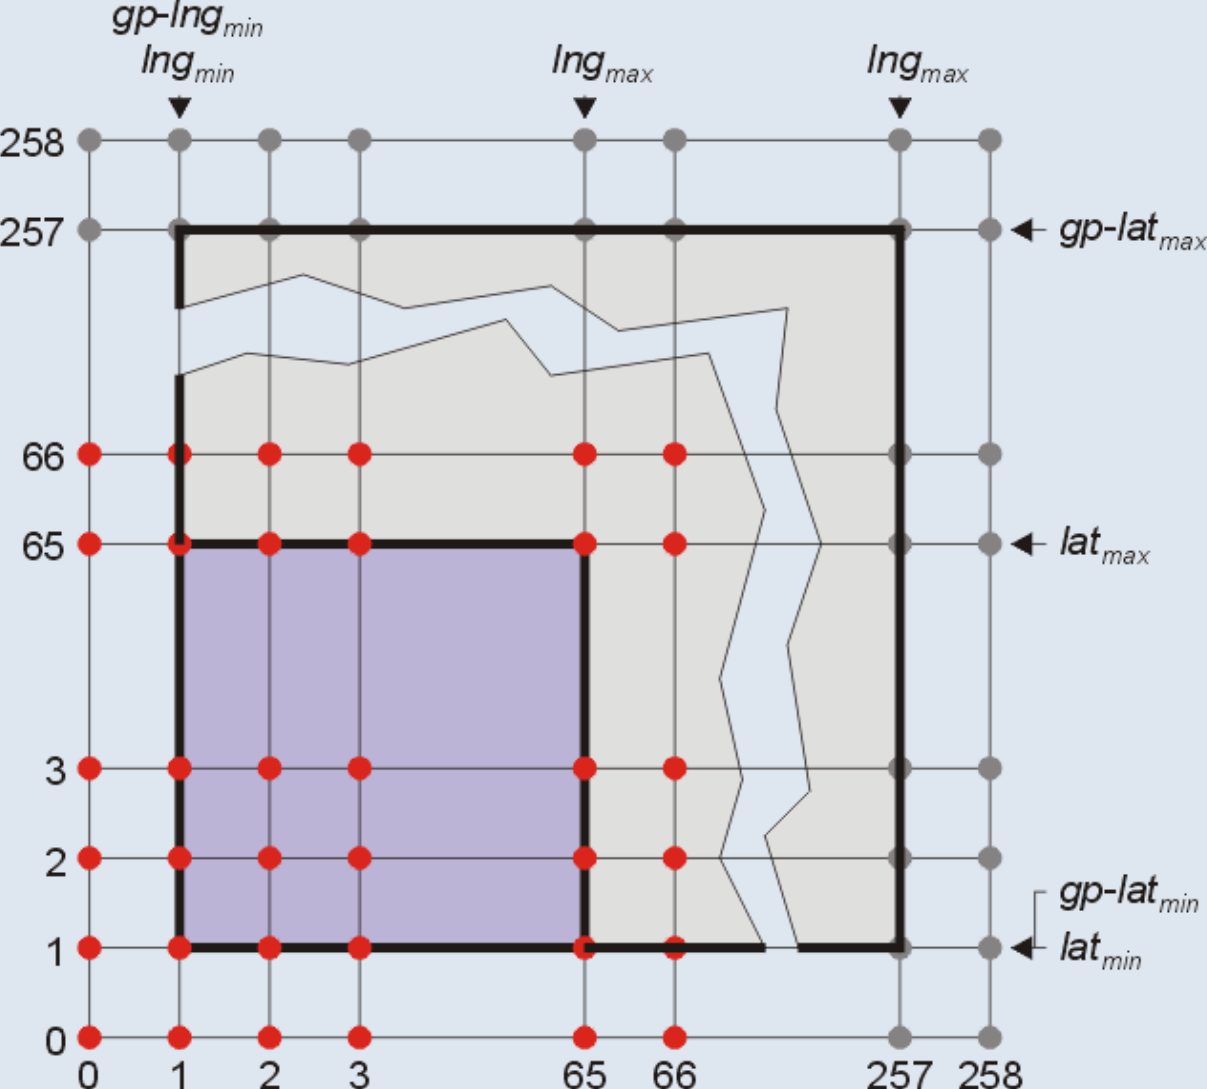
\includegraphics[width=0.5\textwidth]{67_subgrid.png}}
	\caption{67x67 subgrid selection from a grandparent elevation tile.}
\end{figure}

\noindent
The files in the Elev\_mod layer, if present, use the same file format, except that the data block can contain mask flags for individual elevation points to signify that this point is not to be modified. The mask flags are

\begin{itemize}
\item dtype = 8: $\Rightarrow$ mask = UCHAR\_MAX
\item dtype = -16: $\Rightarrow$ mask = SHRT\_MAX
\end{itemize}

\noindent
Note that the 259x259 grid elevation tile resolution is higher than the mesh patch resolution used by Orbiter for that tile (which can be user-defined). If the patch resolution has been set to 64x64 (corresponding to 67x67 including edges and padding) then Orbiter will query a subset of the tile's grandparent node to retrieve the mesh elevation data for that tile. This arrangement allows to reduce the number of files required for the elevation layer.


\subsubsection{Label tile format}
\label{sssec:label_tile_format}
Files in the Label quadtree layer are text files in UTF-8 format and have file extension .lab.\\
Each label file contains the position and labels of surface features within the confines of the corresponding tile to be displayed at a given resolution level when the user enables surface labels in Planetarium mode (\Ctrl+\keystroke{F9}) in Orbiter.\\
Each line in the file describes one label. The format for each label entry is

\begin{lstlisting}[language=OSFS]
<type-id> <latitude> <longitude> <elevation> <label>
\end{lstlisting}

\noindent
where <\textit{type-id}> is a character defining the feature type, <\textit{latitude}> and <\textit{longitude}> are the feature's centre coordinates in degrees, <\textit{elevation}> is the feature's elevation relative to the planet reference radius in metres, and <\textit{label}> is a string describing the feature.\\
<\textit{elevation}> can be set to NaN, in which case Orbiter computes the elevation from its terrain elevation data. This should be avoided if possible to reduce computational cost.\\
The resolution level at which a label appears in the quadtree determines the camera distance at which it appears in the Orbiter render window. By moving a label to a lower resolution level it becomes visible at a greater distance. For example, large cities should be entered at a lower resolution level than small villages.\\
Note that in order to reduce the number of quadtree nodes, Orbiter shifts the resolution visibility by four levels. That is, a label entered in a level-2 tile will become visible when the corresponding level-6 tile is rendered.\\
A label tile file should only contain labels at positions covered by the tile. For example, file\\
\indent Label\textbackslash 05\textbackslash 000000\textbackslash 000001.lab\\
should only contain features with positions 0° $\leq$ lat $\leq$ 90° and -90° $\leq$ lng $\leq$ 0°.\\
To enable the Label layer, the planet's configuration file (Config\textbackslash <\textit{planet-name}>.cfg) must contain the line

\begin{lstlisting}[language=OSFS]
LabelFormat = 2
\end{lstlisting}

\noindent
otherwise the legacy label format is assumed.\\
A label layer for a planet must be accompanied by a label legend file\\
\indent Config\textbackslash <\textit{planet-name}>\textbackslash Label.cfg\\
in UTF-8 format. Each line in the legend file describes a label type, with the format

\begin{lstlisting}[language=OSFS]
<type-id> <default-visible> <marker-id> <r> <g> <b> <type-name>
\end{lstlisting}

\noindent
where <\textit{type-id}> is a character defining the feature type, corresponding to the IDs in the quadtree label files, <\textit{default-visible}> is one of the characters 'x' (visible by default) or 'o' (not visible by default), <\textit{marker-id}> is a character defining the marker shape: 'S' (square, $\Box$), 'O' (circle, $\bigcirc$), 'D' (Delta, $\Delta$) or 'N' (Nabla, $\nabla$). <\textit{r}>, <\textit{g}> and <\textit{b}> are the red, green and blue components (0-255) of the label display colour, and <\textit{type-name}> is a string describing the label type.\\
The user can activate and deactivate the display of specific label types by opening the Planetarium dialog (\Ctrl+\keystroke{F9}) in Orbiter, enabling \textit{Surface Markers}, and opening the \textit{Surface Marker Config} list to select label types.\\
Note that Surface base and Navaid markers are currently not included in the quadtree Label layer. They are generated automatically from parsed Base configuration files and the navaid list in the planet's configuration file.



\subsubsection{Converting surface base tiles}
The main difference in the definition of surface bases between Orbiter releases 2010 and 2016 is the fact that base tiles (surface textures that provide high-resolution texture content in the vicinity of the base) are no longer supported. Base tiles must now be defined directly in the planet's tile quadtree structure.\\
The legacy base tile format consisted of individual tile files in the Textures folder with the naming format\\
\indent <\textit{planet-name}>\_<\textit{res}>\_<\textit{lng-id}>\_<\textit{lat-id}>.dds\\
where <\textit{res}> defines the base tile resolution m ($\geq$ 1), <\textit{lng-id}> is the langitude identifier string, starting with 'W' (west) or 'E' (east) followed by a 4-digit index ($\geq$ 0), and <\textit{lat-id}> is the latitude identifier string, starting with 'N' (north) or 'S' (south) followed by a 4-digit index ($\geq$ 0), e.g.\\
\indent Earth\_2\_W0462\_N0161.dds\\
The relationship between the base tile resolution designation m and the quadtree resolution level n is given by\\
\indent \textit{n} = \textit{m} + 12\\
At base tile resolution level m, the global planet surface map can be considered to be divided into a grid of 2$^{m+9}$ longitude strips and 2$^{m+8}$ latitude strips, with longitude ID strings (from 180° W to 180° E)\\
\indent [W2$^{m+8}$, ... , W0001, E0000, E2$^{m+8}$-1]\\
and latitude ID strings (from 90° S to 90° N)\\
\indent [S2$^{m+7}$, ... , S0001, N0000, N2$^{m+7}$-1]\\
(Note that there are no base tile designations W0000 or S0000). Therefore, mapping base tile longitude designations to quadtree longitude indices is given by:\\
\indent Western hemisphere: W\textit{x} $\rightarrow$ 2$^{m+8}$ - \textit{x}\\
\indent Eastern hemisphere: E\textit{x} $\rightarrow$ 2$^{m+8}$ + \textit{x}\\
and mapping base tile latitude designations to quadtree latitude indices is given by:\\
\indent Northern hemisphere: N\textit{x} $\rightarrow$ 2$^{m+7}$ - 1 - \textit{x}\\
\indent Southern hemisphere: S\textit{x} $\rightarrow$ 2$^{m+7}$ - 1 + \textit{x}\\
For example, base tile Earth\_2\_W0462\_N0161.dds would translate to quadtree tile\\
\indent Earth\textbackslash Surf\textbackslash 14\textbackslash 000350\textbackslash 000562.dds\\
Note that the surface tiles in the quadtree are expected to be size 512x512. The base tiles may be present in various resolutions. This has to be taken into account during the conversion. For example, if base tile Earth\_2\_W0462\_N0161.dds is a 1024x1024 texture, it must be split into four 512x512 tiles which are then stored one level up in the quadtree:\\
\indent Earth\textbackslash Surf\textbackslash 15\textbackslash 000700\textbackslash 001124.dds\\
\indent Earth\textbackslash Surf\textbackslash 15\textbackslash 000700\textbackslash 001125.dds\\
\indent Earth\textbackslash Surf\textbackslash 15\textbackslash 000701\textbackslash 001124.dds\\
\indent Earth\textbackslash Surf\textbackslash 15\textbackslash 000701\textbackslash 001125.dds\\
(A version of the original tile downsized to 512x512 should also be added as Earth\textbackslash Surf\textbackslash 14\textbackslash 000350\textbackslash 000562.dds).\\
If Earth\_2\_W0462\_N0161.dds is a 256x256 texture, it can't be directly converted into a quadtree tile. The following options are available:\\
a) If the appropriate neighbour base tiles are available - in this case,\\
\indent Earth\_2\_W0463\_N0161.dds,\\
\indent Earth\_2\_W0462\_N0160.dds,\\
\indent Earth\_2\_W0463\_N0160.dds,\\
they can be combined into a single 512x512 quadtree tile and stored one resolution level down, as\\
\indent Earth\textbackslash Surf\textbackslash 13\textbackslash 000175\textbackslash 000281.dds.\\
b) The texture can be interpolated to size 512x512 using an image processing utility and then saved as a quadtree tile. This option is less than ideal because the tile is then lacking the high-frequency content supported at that resolution level.\\
c) The 256x256 base tile can be copied into the appropriate quadrant of the original Earth\textbackslash Surf\textbackslash 13\textbackslash 000175\textbackslash 000281.dds parent quadtree tile, if it exists.\\
Note that the base tiles may need to be edited to colour-match the underlying lower-resolution quadtree tiles to provide a seamless transition. Histogram-matching algorithms can be useful here.


\subsection{Planet modules}
\label{ssec:planet_module}
Planet modules can be used to control the motion of a planet (or any other celestial body, such as a moon, the sun, or an asteroid) within the solar system. This allows to implement sophisticated analytic ephemerides solutions which take into account perturbations from other celestial objects.\\
Planets which are not controlled via a DLL module are updated directly by Orbiter. Depending on the settings in the definition file, Orbiter either uses an unperturbed 2-body approximation, resulting in a conic section trajectory (e.g. an ellipse), or uses a dynamic update procedure based on the gravitational forces acting on the planet. Both methods have limitations: the 2-body approach ignores perturbations and is only valid if no massive bodies other than the orbit reference object are nearby. The dynamic update accumulates numerical errors over time, causing the orbits slowly to diverge from the correct trajectories.\\
By using a planet module, analytic perturbation solutions can be used which avoid the short-comings of the methods described above. Perturbation solutions typically describe the perturbed orbit of a planet by expressing the state vectors as a trigonometric series. These series are valid over a limited period of time, after which they start to diverge. Examples of perturbation solutions used in Orbiter are the VSOP87 solution for the 8 major planets and the sun, or the ELP2000 solution for the moon.\\
Planet modules can also define an atmosphere model for the celestial body. Atmosphere models return atmospheric data (temperature, density and pressure) at a specified altitude (and other optional parameters, such as geographic position and time). Atmospheric models can be implemented either directly in the planet module, or in a separate plugin module. Putting the atmosphere model into a separate plugin makes it easier to swap models later.\\
The following sections give a brief introduction into the design of planet modules. A general knowledge of writing orbiter plugins is assumed.

\subsubsection{First steps}
Create a new DLL project for your planet module, e.g. in \textit{Orbitersdk\textbackslash samples\textbackslash MyPlanet}. Set up all the usual include and library paths for Orbiter plugins. Add \textit{orbiter.lib} and \textit{orbitersdk.lib} as additional dependencies.

\subsubsection{The CELBODY2 interface class}
The communication between the Orbiter core and the planet module is performed via callback functions defined in the \textit{CELBODY} and \textit{CELBODY2} classes. (\textit{CELBODY2} is derived from \textit{CELBODY} and contains all the properties of the base class, plus a significantly extended atmospheric parameter interface). The \textit{CELBODY} interface is retained for backward compatibility, but all new planet modules should refer to the \textit{CELBODY2} interface.\\
We now need to the class interface for the new planet module by deriving a custom class from \textit{CELBODY2}. Create a new header file in your project, e.g. \textit{MyPlanet.h}, and add the following:

\begin{lstlisting}
#include "OrbiterAPI.h"
#include "CelbodyAPI.h"

class DLLEXPORT MyPlanet:public CELBODY2
{
	public:
		MyPlanet( OBJHANDLE hObj );
		void clbkInit( FILEHANDLE cfg );
		int clbkEphemeris( double mjd, int req, double* ret );
		int clbkFastEphemeris( double simt, int req, double* ret );
};
\end{lstlisting}

\noindent
\textit{OrbiterAPI.h} contains the general API interface, and \textit{CelbodyAPI.h} contains the planet module-specific interface, in particular the \textit{CELBODY}, \textit{CELBODY2} and \textit{ATMOSPHERE} classes.\\
The \textit{clbkEphemeris} and \textit{clbkFastEphemeris} methods are callback functions which Orbiter will call whenever the planet positions and velocities ("ephemerides") need to be updated. They will be described in more detail below. The clbkInit method is called by Orbiter after the planet module has been loaded. It receives a file handle for the planet's configuration file. This allows the module to read configuration parameters from the file.\\
%TODO reference API manual?
The \textit{CELBODY2} interface contains a few more methods related to defining an atmospheric model. These will be discussed below. Check the API Reference manual for a complete list of class methods.\\
To implement the methods in our \textit{MyPlanet} class, create a source file in your project, e.g. \textit{MyPlanet.cpp}. Add the following lines:

\begin{lstlisting}
#define ORBITER_MODULE
#include "MyPlanet.h"

MyPlanet::MyPlanet( OBJHANDLE hObj ):CELBODY2( hObj )
{
	// add constructor code here
}

void MyPlanet::clbkInit( FILEHANDLE cfg )
{
	/*
	read parameters from config file (e.g. tolerance limits, etc)
	perform any required initialisation (e.g. read perturbation
		terms from data files)
	*/
}

bool MyPlanet::bEphemeris() const
{
	return true;
	// class supports ephemeris calculation
}

int clbkEphemeris( double mjd, int req, double* ret )
{
	// return planet position and velocity for Modified Julian date mjd in ret
}

int clbkFastEphemeris( double simt, int req, double* ret )
{
	/*
	return interpolated planet position and velocity
		for simulation time simt in ret
	*/
}
\end{lstlisting}

\noindent
The first line defining \textit{ORBITER\_MODULE} is required to ensure that all initialisation functions are properly called by Orbiter.\\
\textit{clbkEphemeris} and \textit{clbkFastEphemeris} are the functions which will contain the actual ephemeris calculations for the planet at the requested time. \textit{clbkEphemeris} is only called by Orbiter if the planet's state at an arbitrary time is required (for example by an instrument calculating the position at some future time). When Orbiter updates the planet's position for the next simulation time frame, the \textit{clbkFastEphemeris} function will be called instead. This means that \textit{clbkFastEphemeris} will be called at each frame, each time advancing the time by a small amount. This can be used for a more efficient calculation. Instead of performing a full series evaluation, which can be lengthy, you may implement an interpolation scheme which performs the full calculation only occasionally, and interpolates between these samples to return the state at an intermediate time.\\
For both functions, the requested type of data is specified as a group of \textit{EPHEM\_xxx} bitflags in the \textit{req} parameter. This can be any combination of position and velocity data for the celestial body itself and/or the barycentre of the system defined by the body and all its children (moons). The functions should calculate all required data, either in cartesian or polar coordinates, and fill the \textit{ret} array with the results. \textit{ret} contains 12 entries, used as follows:

\begin{itemize}
\item ret[0-2] $\Rightarrow$ true position
\item ret[3-5] $\Rightarrow$ true velocity
\item ret[6-8] $\Rightarrow$ barycentric position
\item ret[9-11] $\Rightarrow$ barycentric velocity
\end{itemize}

\noindent
Only the fields requested by \textit{req} need to be filled. In cartesian coordinates, the position fields must contain the x, y and z coordinates in [m], and the velocity fields must contain the velocities d\textit{x}/d\textit{t}, d\textit{y}/d\textit{t}, d\textit{z}/d\textit{t} in [m/s]. In spherical polar coordinates, the position fields must contain longitude $\phi$ [rad], latitude $\theta$ [rad] and radial distance \textit{r} [AU], and the velocity fields must contain the polar velocities d$\phi$/dt [rad/s], d$\theta$/dt [rad/s] and d\textit{r}/d\textit{t} [AU/s].\\
The functions should indicate the fields actually calculated via the return value. This is in particular important if not all requests could be satisfied (e.g. position and velocity was requested, but only position could be calculated). The return value is interpreted as a bitflag that can contain the same \textit{EPHEM\_xxx} flags as the \textit{req} parameter. If all requests could be satisfied, it should be identical to \textit{req}. In addition, the return value should contain additional flags indicating the properties of the returned data, including \textit{EPHEM\_POLAR} if the data are returned as spherical polar coordinates, or \textit{EPHEM\_TRUEISBARY} if the true and barycentric coordinates are identical (i.e. the celestial body does not have child bodies).


\subsubsection{The API interface}
Next, we need to define the API interface that will allow Orbiter to load an instance of the celestial body interface. This is done by implementing the \textit{InitInstance} and \textit{ExitInstance} functions in \textit{MyPlanet.cpp}:

\begin{lstlisting}
DLLCKBK CELBODY* InitInstance( OBJHANDLE hBody )
{
	// instance initialisation
	return new MyPlanet;
}

DLLCLBK void ExitInstance( CELBODY* body )
{
	// instance cleanup
	delete (MyPlanet*)body;
}
\end{lstlisting}

\noindent
\textit{InitInstance} and \textit{ExitInstance} are called by Orbiter each time an instance of the planet is loaded or discarded. There are also functions \textit{InitModule} and \textit{ExitModule}, which are called only once per simulation run, and can be used to initialise and clean up global resources:

\begin{lstlisting}
DLLCLBK void InitModule( HINSTANCE hModule )
{
	// module initialisation
}

DLLCLBK void ExitModule( HINSTANCE hModule )
{
	// module cleanup
}
\end{lstlisting}

\noindent
Because usually only a single instance of a specific planet object is created during a simulation, the difference between \textit{InitInstance} and \textit{InitModule} is not as significant here as it is for vessel modules. The \textit{InitModule} and \textit{ExitModule} methods can be omitted if the module doesn't need any global parameter initialisation.


\subsection{Defining an atmosphere}
Planetary atmospheres have a significant influence on the flight behavior of spacecraft. The primary atmospheric parameters are temperature, pressure and density as a function of altitude.\\
Defining a simple atmospheric model is possible by setting a few parameters in the planet's configuration file. More sophisticated models must be coded in the planet's DLL module.\\
Orbiter currently does not model local atmospheric perturbations (climatic/weather effects), although local temperature and pressure variations can be implemented by customised atmosphere models.


\subsubsection{A simple atmosphere}
To define a simple exponentially decaying atmosphere, define the following items in the planet's configuration (.cfg) file:

\begin{itemize}
\item AtmPressure0 $\Rightarrow$ The static atmospheric pressure [Pa] at altitude zero, $p_{0}$.
\item AtmDensity0 $\Rightarrow$ The atmospheric density [kg/m$^{3}$] at altitude zero, $\rho_{0}$.
\item AtmAltLimit $\Rightarrow$ The altitude above which atmospheric effects can be neglected.
\end{itemize}

\noindent
where altitude zero is defined as distance \textit{Size} (as defined in the configuration file) from the planet's centre.\\
The pressure and density at any altitude h is then calculated by Orbiter as

\[ p =
\left\{
\begin{array}{ll}
	p_{0}e^{-Ch} & h \leq AtmLimit \\
	0 & otherwise \\
\end{array} 
\right. \]

\[ \rho =
\left\{
\begin{array}{ll}
	\rho_{0}e^{-Ch} & h \leq AtmLimit \\
	0 & otherwise \\
\end{array} 
\right. \]

\noindent
where $C = \frac{\rho_{0}}{p_{0}}g_{0}$, and $g_{0}$ is the gravitational acceleration at altitude zero.\\
This model assumes constant temperature.


\subsubsection{A more sophisticated atmosphere}
Where the simple model described above is not adequate, a more detailed atmospheric model can be implemented in a plugin module. This section assumes that a module for the celestial body has already been created, as outlined in section \ref{ssec:planet_module}.\\
The atmosphere model interface is described by the \textit{ATMOSPHERE} class defined in \textit{CelbodyAPI.h}. To create a custom atmosphere model, create a new header file in your planet project, e.g. \textit{MyAtmosphere.h}. The atmosphere class interface should look like

\begin{lstlisting}
#include "OrbiterAPI.h"
#include "CelbodyAPI.h"

class DLLEXPORT MyAtmosphere: public ATMOSPHERE
{
	public:
		MyAtmosphere( CELBODY2* body );
		const char* clbkName() const;
		bool clbkConstants( ATMCONST* atmc ) const;
		bool clbkParams( const PRM_IN* prm_in, PRM_OUT* prm_out );
};
\end{lstlisting}

\noindent
The constructor takes the \textit{CELBODY2} class instance of the associated celestial body as a parameter.\\
The \textit{clbkName} callback function should return a short name identifying the model.\\
\\
The \textit{clbkConstants} callback function should return in \textit{atmc} some basic atmosphere parameters, such as the mean density and pressure at ground level, gas constant and ratio of specific heats, as well as some rendering parameters.\\
Note that some of the parameters returned by \textit{clbkConstants} may be overwritten by the settings defined in the celestial body's configuration file. Configuration file entries take precedence over \textit{clbkConstants}.\\
The \textit{clbkParams} callback function should return atmospheric temperature, density and pressure at the location specified by the data in the \textit{prm\_in} parameter. Simple models may depend on altitude only, but more sophisticated models can make use of the additional parameters such as position (longitude and latitude), solar flux, geomagnetic index, and date.\\
Create a source file, e.g. \textit{MyAtmosphere.cpp}, to implement the actual model. A very simplistic implementation may look like this:

\begin{lstlisting}
#include "MyAtmosphere.h"

static double T0       = 288.0;  // ground level temperature [K]
static double p0       = 101325; // ground level pressure [Pa]
static double rho0     = 1.2250; // ground level density [kg/m^3]
static double R        = 286.91; // gas constant
static double gamma    = 1.4;    // ratio of specific heats
static double altlimit = 200e3;  // cutoff altitude
static double C        = rho0 / p0;

MyAtmosphere::MyAtmosphere( CELBODY2* body ):ATMOSPHERE( body )
{
}

const char* MyAtmosphere::clbkName() const
{
	static char* name = "Simple";
	return name;
}

bool MyAtmosphere::clbkConstants( ATMCONST* atmc ) const
{
	atmc->p0 = p0;
	atmc->rho0 = rho0;
	atmc->R = R;
	atmc->gamma = gamma;
	atmc->altlimit = altlimit;
	return true;
}

bool MyAtmosphere::clbkParams( const PRM_IN* prm_in, PRM_OUT* prm_out )
{
	double z = (prm_in->flag & PRM_ALT ? prm_in->alt : 0.0);
	if (z < 200e3)
	{
		double scale = exp( -C * z );
		prm_out->T = T0;
		prm_out->rho = rho0 * scale;
		prm_out->p = p0 * scale;
		return true;
	}
	else
	{
		prm_out->T = 0;
		prm_out->rho = 0;
		prm_out->p = 0;
		return false;
	}
}
\end{lstlisting}

\noindent
The above example serves only as an illustration. The actual atmosphere models provided with the Orbiter distribution are more complex. For some background on the supported Earth atmosphere models, see "Earth Atmosphere Model" in Orbiter Technical Reference.\\
Now we need to link the atmosphere model into the celestial body interface. This can be done with the \textit{SetAtmosphere} function of the \textit{CELBODY2} class. Add the following statement to the \textit{clbkInit} method of your \textit{MyPlanet} definition:

\begin{lstlisting}
#include "MyAtmosphere.h"

void MyPlanet::clbkInit( FILEHANDLE cfg )
{
	SetAtmosphere( new MyAtmosphere( this ) );
}
\end{lstlisting}

\noindent
The atmosphere instance will be destroyed automatically when the planet instance is deleted.


\subsubsection{External atmosphere modules}
Instead of implementing the atmosphere model inside the planet module, it can can also be implemented in a separate plugin module. This makes it easier to exchange the atmosphere model for a different one later on, without having to have access to the rest of the planet module code.\\
To implement the atmosphere as a separate module, create a new DLL project for it. Add the \textit{MyAtmosphere.h} and \textit{MyAtmosphere.cpp} files created in the previous section to the project. Since the atmosphere is now defined in its own module, add the line

\begin{lstlisting}
#define ORBITER_MODULE

\end{lstlisting}

\noindent
on top of \textit{MyAtmosphere.cpp}.\\
In addition, you need to define an API interface to the module code. It should look like this:

\begin{lstlisting}
DLLCLBK void InitModule( HINSTANCE hModule )
{
	// module initialisation
}

DLLCLBK void ExitModule( HINSTANCE hModule )
{
	// module cleanup
}

DLLCLBK ATMOSPHERE* CreateAtmosphere( CELBODY2* cbody )
{
	return new MyAtmosphere( cbody );
}

DLLCLBK void DeleteAtmosphere( ATMOSPHERE* atm )
{
	delete (MyAtmosphere*)atm;
}
\end{lstlisting}

\noindent
By convention, external planetary atmosphere modules should be placed in the\\
\indent \textit{Modules\textbackslash Celbody\textbackslash <Name>\textbackslash Atmosphere}\\
folder, where <\textit{Name}> is the celestial body's name. So in our case,\\
\indent \textit{Modules\textbackslash Celbody\textbackslash MyPlanet\textbackslash Atmosphere\textbackslash MyAtmosphere.dll}\\
We now need to modify the \textit{MyPlanet} code to allow it to load its atmosphere interface from an external module. Replace the \textit{SetAtmosphere} statement in the \textit{clbkInit} function with

\begin{lstlisting}
void MyPlanet::clbkInit( FILEHANDLE cfg )
{
	LoadAtmosphereModule( "MyAtmosphere" );
}
\end{lstlisting}

\noindent
However, this causes the atmospheric module name to be hardcoded in the planet module. A more flexible method is to specify the atmospheric module in the celestial body's configuration file, using the \textit{MODULE\_ATM} entry. Our \textit{MyPlanet.cfg} file might look like this:

\begin{lstlisting}[language=OSFS]
NAME = MyPlanet
MODULE = MyPlanet
MODULE_ATM = MyAtmosphere
\end{lstlisting}

\noindent
If the \textit{MODULE\_ATM} entry is defined in the configuration file, then the default \textit{CELBODY2::clbkInit} implementation will load the atmosphere module directly, so we only need to make sure to call the base class method:

\begin{lstlisting}
void MyPlanet::clbkInit( FILEHANDLE cfg )
{
	CELBODY2::clbkInit( cfg );
}
\end{lstlisting}

\noindent
Calling the \textit{CELBODY2::clbkInit} method also enables another interesting feature: Before reading the \textit{MODULE\_ATM} entry in the planet configuration file, Orbiter scans the \textit{Config\textbackslash <Name>\textbackslash Atmosphere.cfg} file for an entry "Model" and uses that, if present. This file is written by the \textit{Atmosphere configuration tool} in the Extra tab of the Orbiter launchpad, which provides a convenient method for users to change atmosphere models. This mechanism allows to add new atmosphere modules without the need to change any configuration files. As long as the atmosphere DLL modules are placed in the correct location (\textit{Modules\textbackslash Celbody\textbackslash <Name>\textbackslash Atmosphere}), they will be scanned automatically by the atmosphere selector tool.


\subsubsection{Adding and replacing atmosphere models}
Most of the celestial body modules in the default Orbiter distribution have built-in support for external atmosphere modules, and some of them (Earth, Mars and Venus) come with one or several atmosphere modules. To add additional choices for atmosphere models for a body, create one as outlined above, and simply drop the DLL library into the \textit{Modules\textbackslash Celbody\textbackslash <Name>\textbackslash Atmosphere} folder. If that folder doesn't exist yet, you have to create it. The user can then select the new model from the Extra tab in the Orbiter Launchpad (Celestial body configuration | Atmosphere configuration).\\
For best support of the atmosphere model selection tool, your atmosphere module should contain two additional API functions:

\begin{lstlisting}
DLLCLBK char* ModelName()
{
	static char* name = "MyAtmosphere";
	return name;
}

DLLCLBK char* ModelDesc()
{
	static char* desc = "My custom atmosphere model";
	return desc;
}
\end{lstlisting}

\noindent
The string returned by the \textit{ModelName} function represents the model in the dialog's selection list box. The string returned by \textit{ModelDesc} should contain a short description (max 256 characters displayed in the dialog box when the model is selected.\\
If you don't want to design your own custom atmosphere model, you can quickly add atmospheres to planets by replicating existing ones. Simply copy an atmosphere module from the\\
\indent \textit{Modules\textbackslash Celbody\textbackslash <Name>\textbackslash Atmosphere}\\
folder of one planet to that of another one. It then becomes available in the list of atmospheres for that planet. Note that the module only provides the physical atmospheric parameters. You will still have to edit the definition file to provide visual effects.\\
Of course, replicating an atmosphere should be regarded as a quick and dirty trick for experimentation. Atmospheres are always tailor-made for specific bodies, and don't realistically fit anywhere else.


\subsubsection{Earth default atmosphere models}
The Orbiter distribution contains three Earth atmosphere models that can be selected by the user from the Extra tab in the Launchpad dialog. See "Earth Atmosphere Model" in Orbiter Technical Reference for further details on the different models.\\
\textbf{Jacchia71-Gill Atmosphere Model.} This is an implementation of the Jacchia-71 (J71) model\cite{jacchia71}, using a polynomial series approximation by Gill\cite{gill96}. It uses a static US Standard Atmosphere model below 90km, and a diffusion-equilibrium solution be­tween 90 and 2500km altitude. The only model parameter is the exospheric temperature.\\
\textbf{NRLMSISE-00 Atmosphere Model.} This model is based on the MSISE90 model, with the addition of further corrections based on observation data. MSISE90 provides the neutral temperature and density from ground level to thermospheric altitudes. Unlike the Jacchia models, the low-altitude data are not static, but vary with location.\\
\textbf{Orbiter 2006 Legacy model.} This is the model that was used in the Orbiter 2006 Edition. It is based on a static standard model\cite{anderson2000} below 105km, and assumes constant temperature and exponentially decaying density and pressure between 105 and 200km. This model underestimates density and pressure above $\sim$120km, which reduces the orbit decay of object in low Earth orbit.\\
In addition, the atmosphere can be disabled for testing/debugging purposes.

\subsubsection{Mars atmosphere}
Orbiter uses the following atmospheric parameter profiles for Mars:

%\begin{table}[H]
	%\centering
	\begin{longtable}{ |p{0.2\textwidth}|p{0.1\textwidth}|p{0.1\textwidth}|p{0.1\textwidth}|p{0.1\textwidth}|p{0.1\textwidth}|p{0.1\textwidth}| }
	\hline\rule{0pt}{2ex}
	Altitude [km] & 0 & 2 & 4 & 14 & 20 & 30\\
	\hline\rule{0pt}{2ex}
	Temperature [K] & 195 & 200 & 200 & 180 & 180 & 165\\
	\hline\rule{0pt}{2ex}
	Pressure [Pa] & 610.0 & 499.5 & 410.1 & 145.1 & 75.2 & 23.9\\
	\hline\rule{0pt}{2ex}
	Density [kg m$^{-3}$] & 0.02 & 0.0160 & 0.0131 & 0.0052 & 2.7$\cdot$10$^{-3}$ & 9.3$\cdot$10$^{-4}$\\
	\hline
	\end{longtable}
%\end{table}

\noindent
\begin{figure}[H]
	\centering
	\subfigure{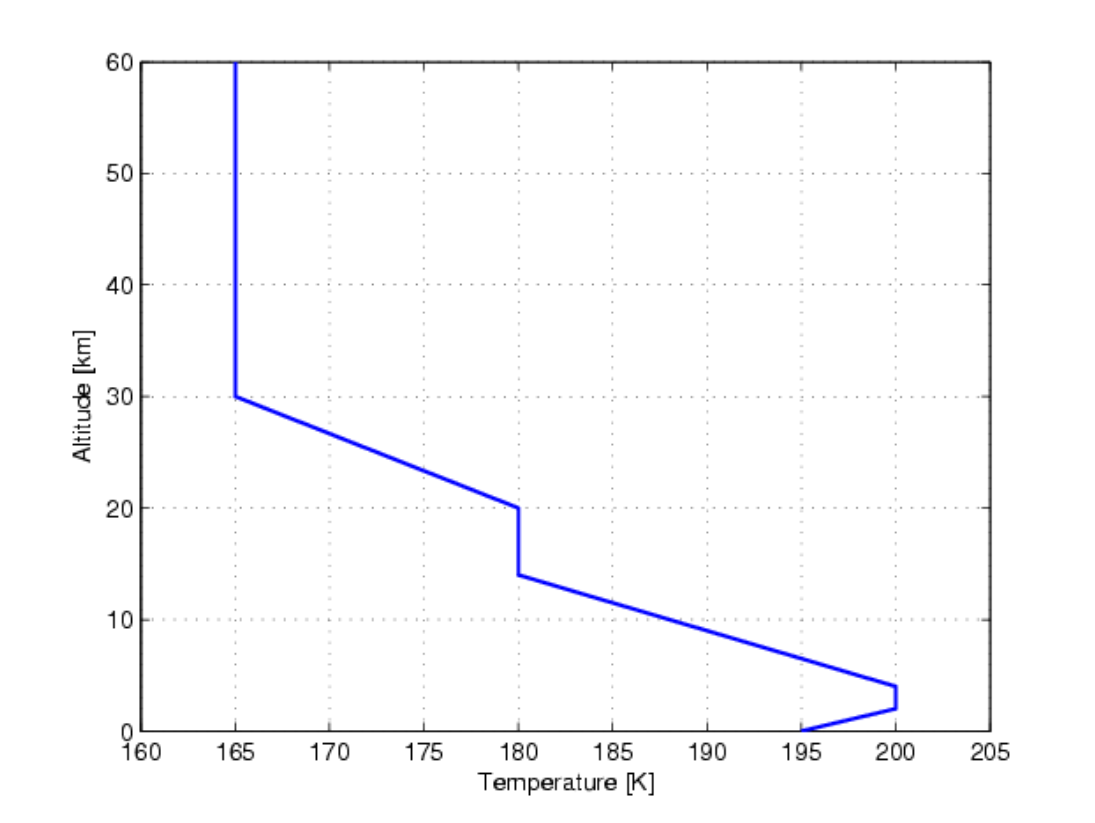
\includegraphics[width=0.49\textwidth]{mars_atm_temperature.png}}
	\subfigure{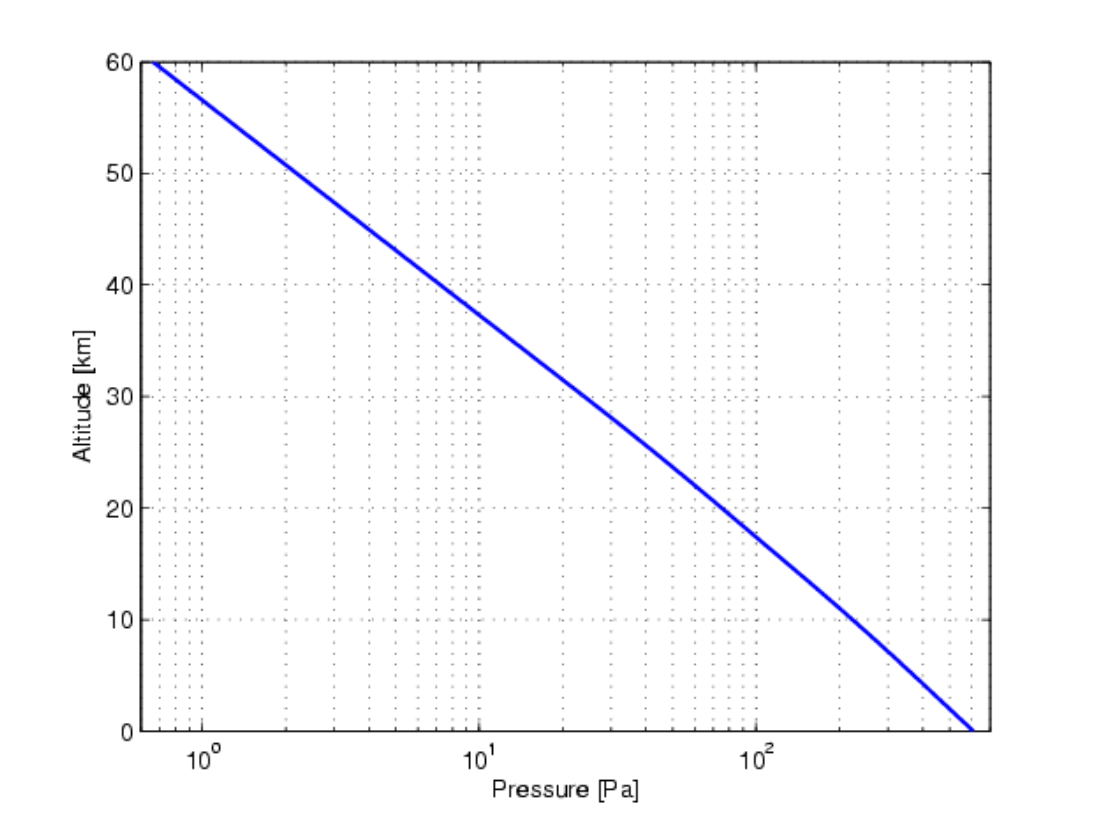
\includegraphics[width=0.49\textwidth]{mars_atm_pressure.png}}
	\subfigure{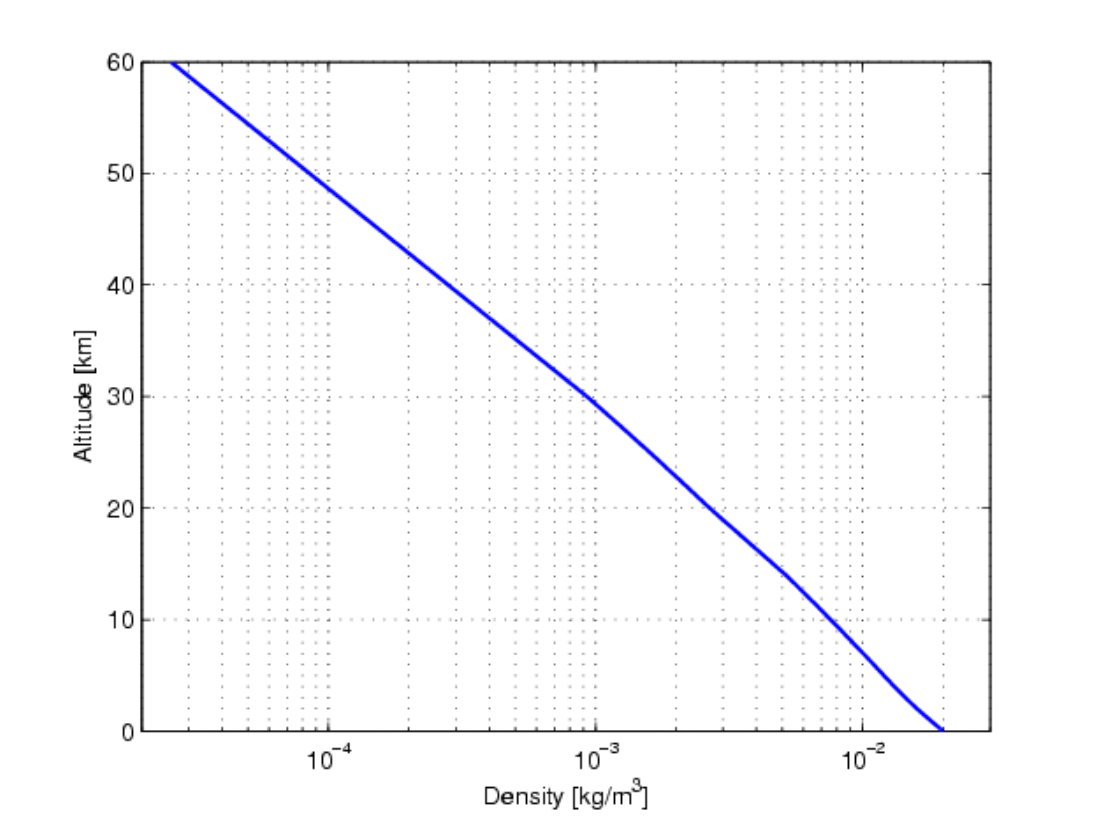
\includegraphics[width=0.49\textwidth]{mars_atm_density.png}}
\end{figure}

\noindent
Atmospheric parameters:

\begin{itemize}
\item Surface pressure: $p_{0}$ = 610.0 Pa
\item Surface density: $\rho_{0}$ = 0.020 kg m$^{-3}$
\item Ratio of specific heats: $\gamma$ = 1.2941
\item Specific gas constant: \textit{R} = 188.92 J K$^{-1}$ kg$^{-1}$
\end{itemize}

\noindent
Orbiter defines the upper atmosphere altitude limit as 100 km.


\subsubsection{Venus atmosphere}
Orbiter uses the following atmospheric parameter profiles for Venus:

%\begin{table}[H]
	%\centering
	\begin{longtable}{ |p{0.2\textwidth}|p{0.1\textwidth}|p{0.1\textwidth}|p{0.1\textwidth}|p{0.1\textwidth}|p{0.1\textwidth}|p{0.1\textwidth}| }
	\hline\rule{0pt}{2ex}
	Altitude [km] & 0 & 30 & 60 & 70 & 90 & 200\\
	\hline\rule{0pt}{2ex}
	Temperature [K] & 750 & 480 & 230 & 230 & 180 & 180\\
	\hline\rule{0pt}{2ex}
	Pressure [Pa] & 9.2M & 897k & 14.2k & 1.85k & 18.5 & 3.4$\cdot$10$^{-11}$\\
	\hline\rule{0pt}{2ex}
	Density [kg m$^{-3}$] & 65 & 9.9 & 0.33 & 0.043 & 5.4$\cdot$10$^{-4}$ & 1.0$\cdot$10$^{-15}$\\
	\hline
	\end{longtable}
%\end{table}

\noindent
\begin{figure}[H]
	\centering
	\subfigure{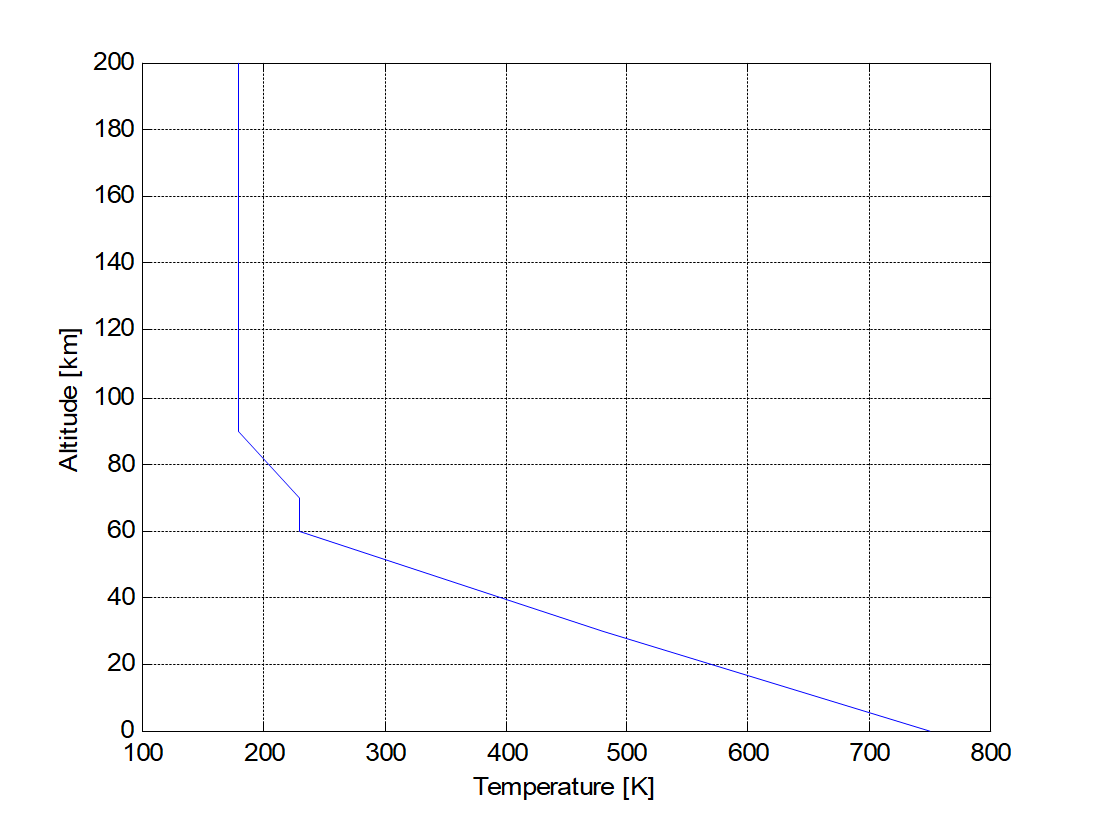
\includegraphics[width=0.49\textwidth]{venus_atm_temperature.png}}
	\subfigure{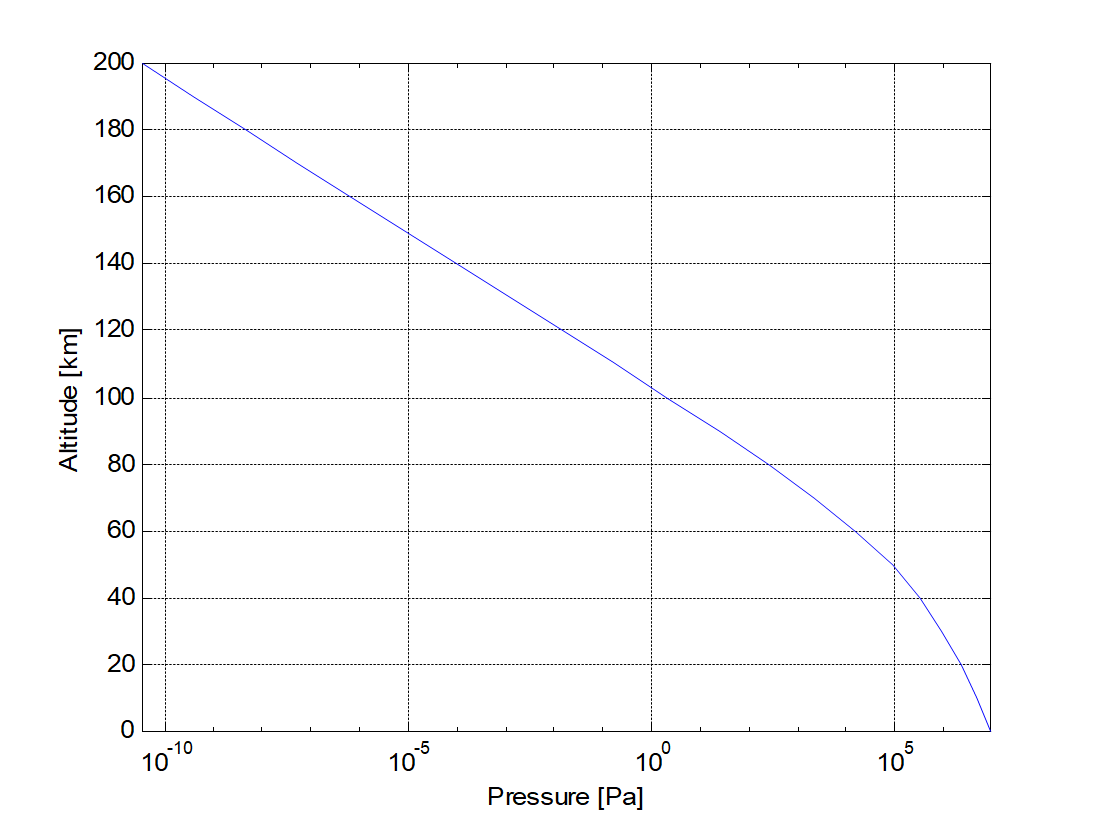
\includegraphics[width=0.49\textwidth]{venus_atm_pressure.png}}
	\subfigure{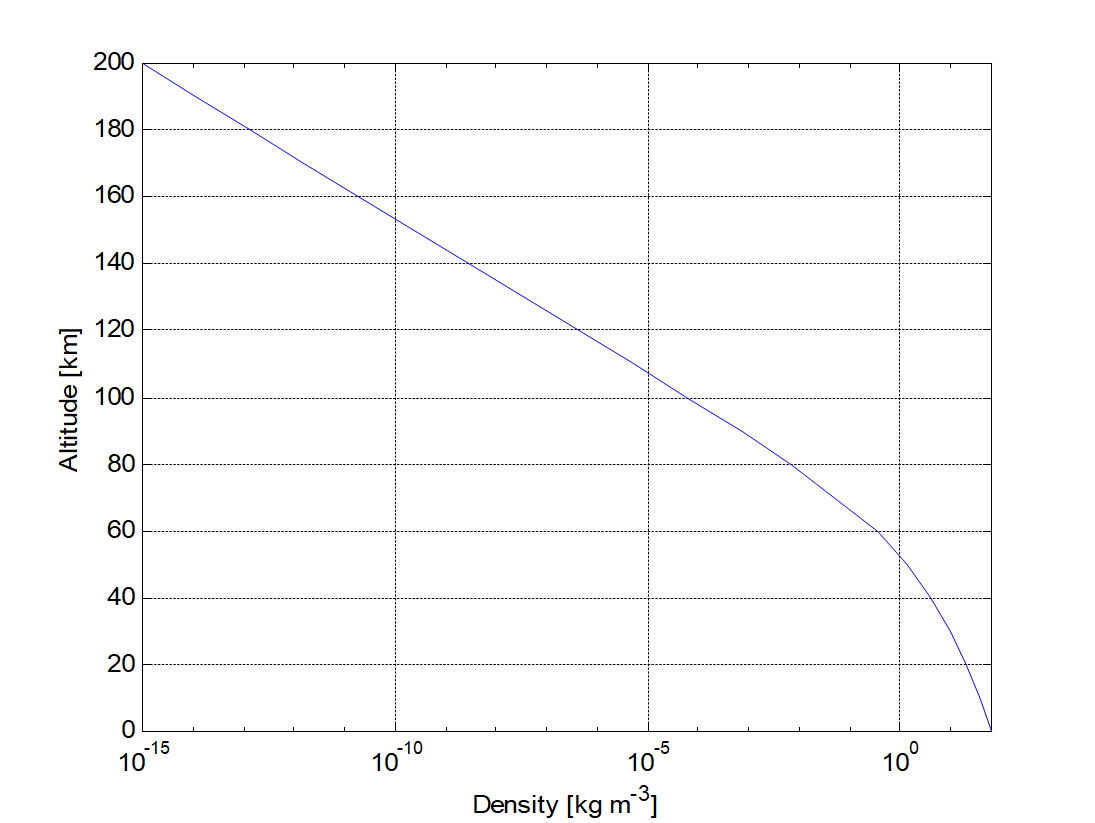
\includegraphics[width=0.49\textwidth]{venus_atm_density.png}}
\end{figure}

\noindent
Atmospheric parameters:

\begin{itemize}
\item Surface pressure: $p_{0}$ = 9.2 MPa
\item Surface density: $\rho_{0}$ = 65 kg m$^{-3}$
\item Ratio of specific heats: $\gamma$ = 1.2857
\item Specific gas constant: \textit{R} = 188.92 J K$^{-1}$ kg$^{-1}$
\end{itemize}

\noindent
Orbiter defines the upper atmosphere altitude limit as 200 km. The cloud layer is set at an altitude of 60 km.


\subsubsection{The speed of sound}
Orbiter uses the equation for an ideal gas to compute the speed of sound as a function of absolute temperature:

\[ a = \sqrt{\gamma RT} \]

\noindent
where $\gamma$ is the ratio of specific heat at constant pressure $c_{p}$, and specific heat at constant temperature, $c_{v}$, for the gas, $\gamma = c_{p} / c_{v}$ For air at normal conditions, $\gamma$ = 1.4. This value is used by Orbiter as a default. It can be overridden by setting the \textit{AtmGamma} parameter in the planet's configuration file.\\
\textit{R} is the specific gas constant. By default, Orbiter uses the value for air, 286.91 J K$^{-1}$ kg$^{-1}$. This can be overridden by setting the \textit{AtmGasConstant} parameter in the planet's configuration file.\\
\textbf{Mach number:} The Mach number is an essential parameter in aerodynamics. It expresses a velocity \textit{v} in units of the current speed of sound:

\[ M = \frac{v}{a} \]


\end{document}
